\chapter{Conclusão}
\label{cap:conclusao}

Ao longo deste trabalho de conclusão de curso, realizamos atividades que passam
pelas principais áreas de conhecimento da Engenharia de Software, como a
gerência de projetos, a gerência de configuração de software,
o levantamento e a elaboração de requisitos, a análise e o \textit{design},
a implementação, e aqui incluímos a criação de testes automatizados,
a manutenção e a implantação de uma plataforma real de software livre, dentre
outras.
%
Nos preocupamos em contribuir, na prática, com a escrita de código~\footnote{%
Segue o link de alguns \textit{commits} realizado por nós durante a realização
deste trabalho: \\
\url{https://gitorious.org/noosfero/danielbucher-noosfero/commit/09c1af056d800c0f67632360734004b5c7090b7e}\\
\url{https://gitorious.org/noosfero/danielbucher-noosfero/commit/31298c57b1725da6fdc1b96744cecf232897d80f}},
uma vez que, em nossa visão, esta é a principal missão de um Engenheiro de
Software.
%
Outra atividade que julgamos ser de fundamental importância para a continuidade
deste trabalho, diz respeito ao repasse do conhecimento adquirido para uma
equipe de alunos do curso de Engenharia de Software, que trabalhou inicialmente
no Portal da FGA.


\begin{figure}[h!]
	\centering
	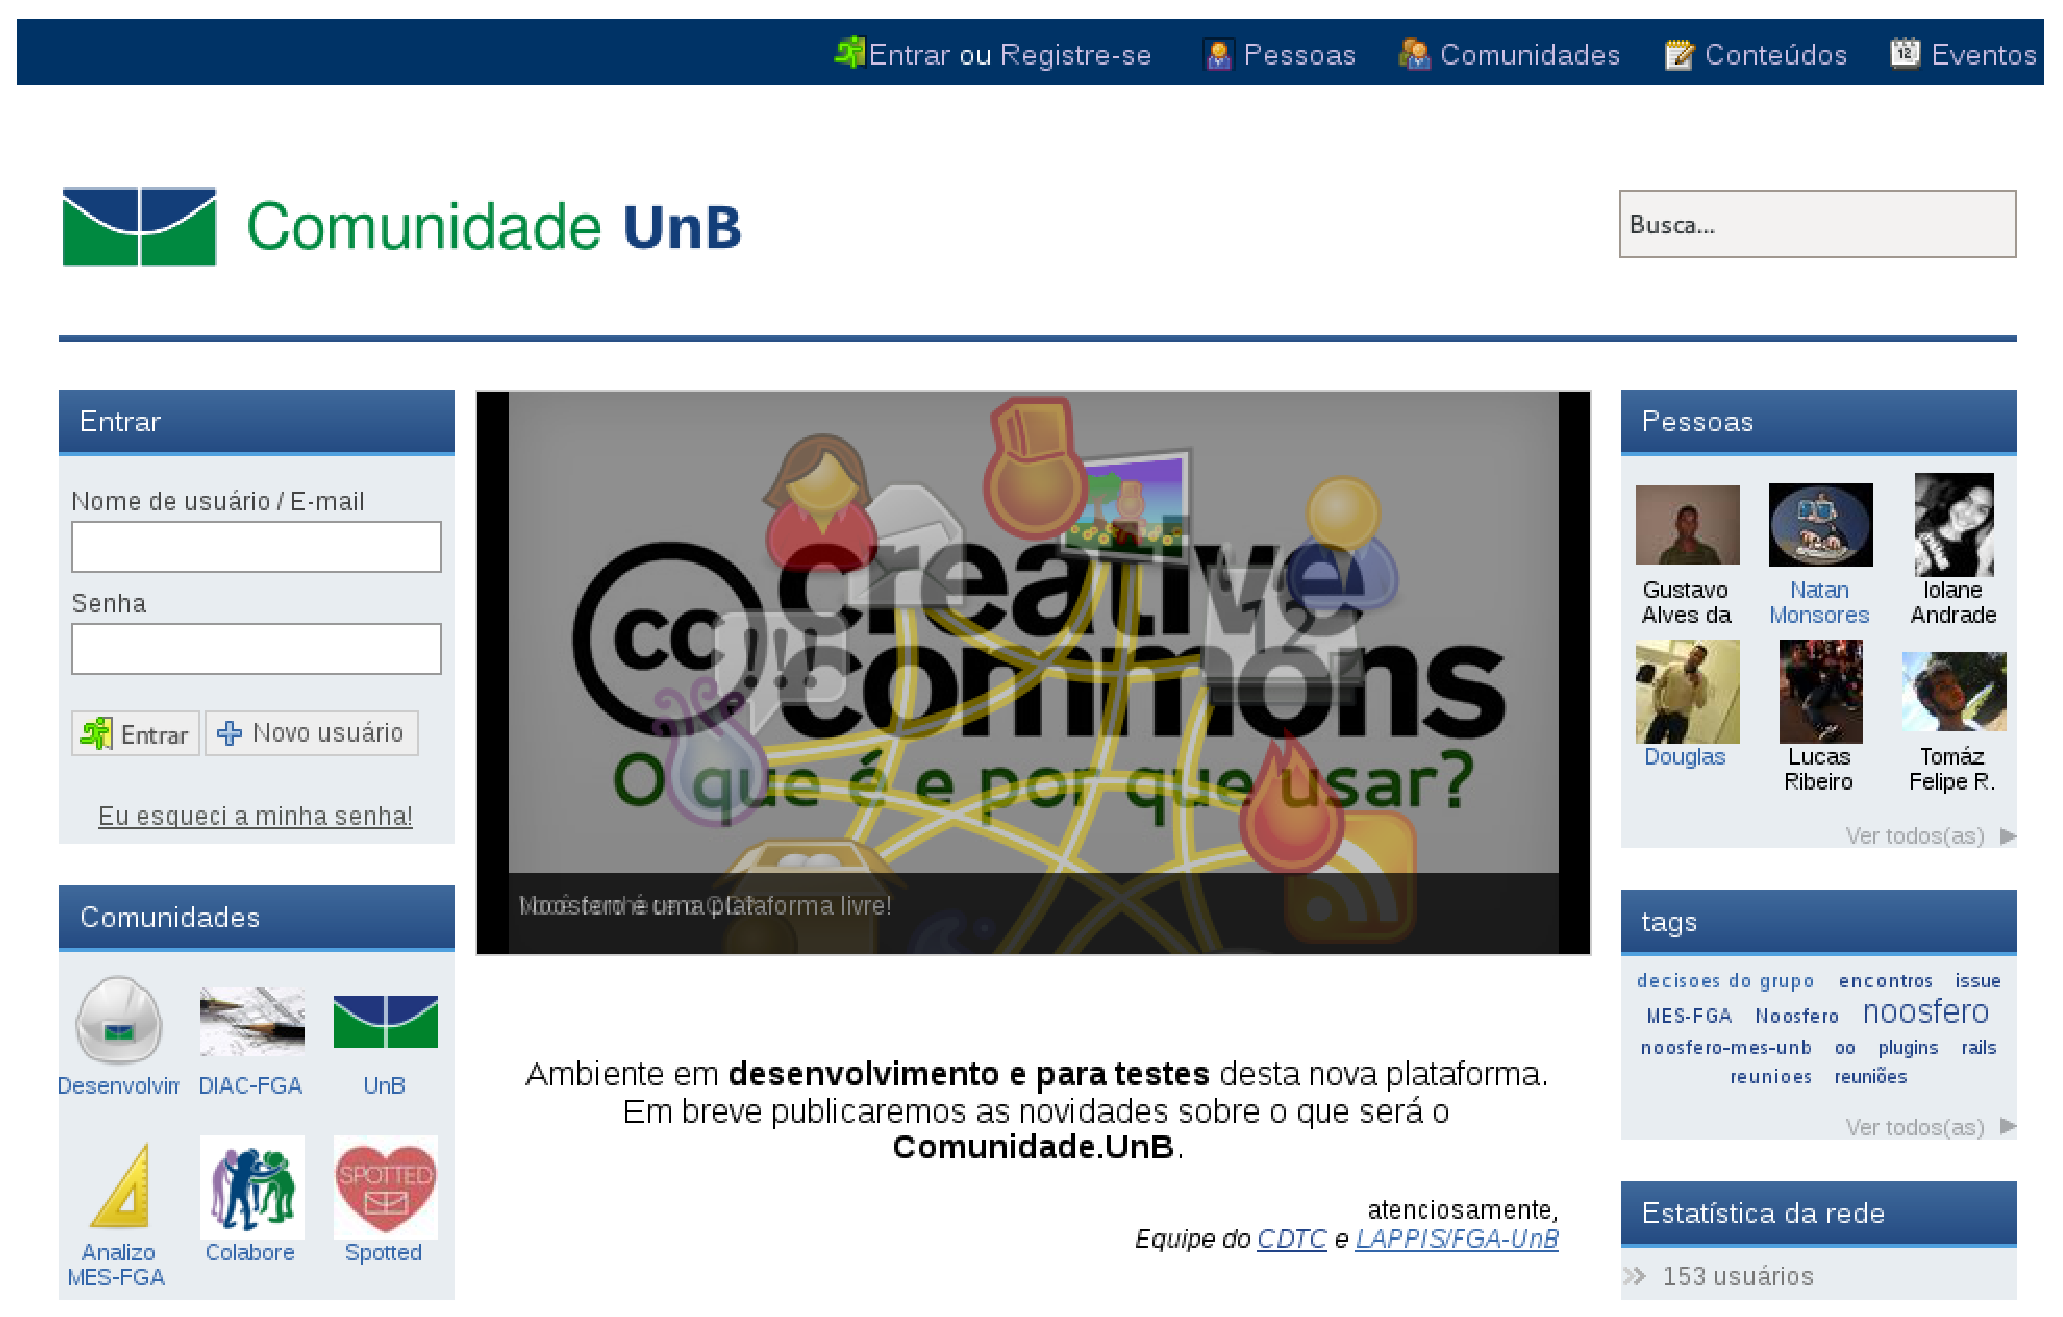
\includegraphics[keepaspectratio=true,scale=0.45]
	  {figuras/comunidade-unb.eps}
	\caption{Tela inicial da Comunidade.UnB}
	\label{homepage:comunidade.unb}
\end{figure}

Esta experiência nos proporcionou a possibilidade de participar de um processo
distribuído de desenvolvimento de software com outras equipes espalhadas pelo
país e de fazer parte de uma comunidade de software livre.
%
Ao final deste trabalho, julgamos que a rede Comunidade.UnB está bem próxima
da capacidade de ser lançada oficialmente para a universidade, graças ao
apoio do CDTC, que viabilizou os contatos necessários para formalizar os
pedidos de uso, por exemplo, das bases de dados existentes nela, e graças
à comunidade do Noosfero que nos apoiou durante sua execução.
%
Por fim, a Figura \ref{homepage:comunidade.unb} apresenta a página inicial do
Comunidade.UnB, ainda em ambiente de testes, que já consta com 153 usuários
e 14 comunidades.

\section{Trabalhos Futuros}
\label{sec:future-works}

Nessa seção, apresentamos alguns trabalhos futuros que podem dar continuidade a
este trabalho. Além de algumas novas funcionalidades para o Noosfero, fizemos
um levantamento sobre alguns protocolos que podem ser usados para implementar a
federação tecnológica para o Noosfero, bem como propomos um estudo sobre
escalabilidade, de forma a conseguir atender um número de requisições
concorrentes elevados para manter um bom nível de desempenho.

\subsection{Federação Tecnológica}

A federação tecnológica é um assunto que tem sido constantemente discutido
na comunidade do Noosfero. A transição do Noosfero para uma rede social federada
é essencial para a criação de um ecossistema de redes de colaboração que
comunicam entre si.
%
A federação consiste na habilidade de redes diferentes de conversarem entre si,
de forma que um usuário da rede Comunidade.UnB, por exemplo, poderia receber
atualizações de uma comunidade em outra rede baseada em Noosfero, ou em
qualquer outra ferramenta que implemente o mesmo protocolo de federação,
através de regras pré-acordadas \cite{prodomou2010}.

Em princípio, a estrutura para redes federadas proposta para a plataforma Noosfero
consistia em um padrão aberto, chamado \textbf{OStatus}
~\footnote{\url{http://www.w3.org/community/ostatus/}}, que foi proposto
por Evan Prodomou para ser utilizado pelo \textbf{StatusNet}~\footnote{\url{%
http://status.net/}}, um servidor  \textit{open-surce} para
\textit{microblogging} escrito em PHP.
%
O OStatus foi construído com base no padrão para criação de \textit{feeds},
\textbf{Atom}~\footnote{\url{http://www.atomenabled.org/}} e no
protocolo \textbf{\textit{PubSubHubbub}}%
~\footnote{\url{https://code.google.com/p/pubsubhubbub/}}(\textbf{PuSH}).
%
O funcionamento do \textbf{OStatus} pode ser resumido da seguinte forma:
os \textit{sites} produzem atualizações no formato de \textit{feeds} através
do padrão \textbf{Atom} e utilizam o protocolo \textbf{PuSH}
para enviar estas atualizações para outros \textit{sites} \cite{OStatusBasics}.
%
Posteriormente, \textbf{OStatus} passou a ser desenvolvido como um
grupo de trabalho da \textit{World Wide Web Consortium} (W3C) e estava no
caminho para se tornar um padrão oficial.

No entanto, em dezembro de 2013, Prodomou declarou que estava desenvolvendo
um novo projeto chamado \textbf{pump.io} quer iria substituir o
\textbf{StatusNEt}~\footnote{\url{http://status.net/2012/12/18/%
upcoming-changes-in-the-status-net-service}} e que utilizará um novo
protocolo para a federação chamado \textbf{Activity Streams}%
~\footnote{\url{http://activitystrea.ms/}} baseado em \textbf{\textit{%
JavaScript Object Notation}} (\textbf{JSON}).
%
Assim, faz-se necessário realizar uma série de estudos e experimentos
antes de tomar a decisão do protocolo a ser adotado, ou mesmo desenvolvido
do início.

Quando a federação tecnológica for uma realidade no Noosfero, existirá a
possibilidade de existir uma ``rede de redes'' de colaboração federadas,
com várias universidades, por exemplo, tendo sua própria rede de colaboração
com sendo um nó.
%
Essa realidade aumentaria consideravelmente o número de requisições sendo
feitas a uma instância do Noosfero em uma universidade, uma vez que o público
fazendo uso desta tecnologia tende a se multiplicar.
%
Desta forma, propomos que seja realizado um estudo sobre a possibilidade
de aumentar a escalabilidade das redes, possivelmente havendo redundância
de hospedeiros, tanto do Noosfero em si, quanto do Varnish, a camada
responsável por atuar como um servidor de \textit{proxy} reverso.

%-----------------------------------------------------------------------------%

\subsection{Próximas funcionalidades}

%------------------------------funcionalidade---------------------------------%
\subsubsection{Convite para participação de comunidades}

Esta funcionalidade prevê melhorias no sistema de convite para participar de
uma comunidade. Hoje, os convites são realizados
exclusivamente através de e-mail, seja entrando com o e-mail da pessoa
diretamente ou pesquisando na lista de contatos de um e-mail passado.
%
Planejamos esta funcionalidade para incluir uma interface através da qual um
usuário possa adicionar facilmente outros usuários da sua lista de amigos,
pesquisando pelo nome, ou, caso deseje convidar um usuário do qual não seja
amigo, ou alguém que ainda não tenha cadastro na rede através do e-mail.

\subsubsubsection*{Histórias de usuário}

\begin{enumerate}

%--------------------------------história-------------------------------------%
\item \underline{Convidar usuários da rede}

	\textbf{Para} facilitar a criação de convites para juntar-se a comunidade

	\textbf{Como} um membro de comunidade com permissão para convidar membros

	\textbf{Eu quero} convidar usuários através de uma interface que busque na lista
	de perfis de pessoas do ambiente e auto-complete conforme for digitando.

\subsubsubsection*{Cenários de uso}

	\begin{enumerate}

		\item \underline{Procurar um usuário cadastrado}

		\textbf{Dado} que eu estou logado com meu usuário

		\textbf{E} meu usuário é administrador do Comunidade.UnB

		\textbf{E} o usuário ``Zé'' existe

		\textbf{E} o usuário ``Zé'' não é membro do Comunidade.UnB

		\textbf{E} eu estou na página de convidar amigos para o Comunidade.UnB

		\textbf{Quando} eu digitar ``Zé'' no campo de convidar novos amigos

		\textbf{Então} eu devo ver um \textit{token}\footnote{Neste contexto, um
		\textit{token} representa um objeto, no caso um perfil de usuário, que possua
		um nome que bata com o campo digitado.} representando o usuário ``Zé''.

	\end{enumerate}


\end{enumerate}

%------------------------------funcionalidade---------------------------------%

\subsubsection{Utilização de SSL}

Esta ``funcionalidade''~\footnote{Colocamos funcionalidade entre aspas pelo
fato de esta não ser composta de histórias de usuários, como as demais, mas sim
de histórias técnicas que precisam ser desenvolvidas para atender a requisitos
não funcionais mencionados na Seção \ref{sec:non-functional-req}.} diz respeito
ao uso de uma camada de SSL e do protocolo HTTPS no Comunidade.UnB.
%
É importante, para manter a integridade das informações
dos usuários, como suas senhas, que as requisições realizadas para o
Comunidade.UnB passem uma uma camada de criptografia, conforme mencionado em
\ref{sec:non-functional-req}.
%
Para tanto, já foi proposto na lista de discussão do Noosfero a
utilização da ferramenta \textbf{Pound}~\footnote{\url{http://www.apsis.ch/pound}}
para atuar como um \textit{front-end} de HTTPS para o \textbf{Apache}.
%
No entanto, seria necessário a aquisição de um certificado SSL~\footnote{\url{%
http://en.wikipedia.org/wiki/Transport_Layer_Security}} que fosse suportado
pelos navegadores mais utilizados.
%
A história apresentada nesta sub-seção é descrita como uma história técnica ao
invés de uma história de usuário, uma vez que o objetivo desta é atender a
um requisito não-funcional do sistema.

\begin{enumerate}


%--------------------------------história-------------------------------------%
\item \underline{Conexão criptografada}

	\textbf{Para} evitar o roubo de informação pessoal dos usuários do
Comunidade.UnB

	\textbf{Como} um responsável pela manutenção do Comunidade.UnB

	\textbf{Eu quero} que as requisições feitas à rede utilizem o protocolo
HTTPS.

%-----------------------------------------------------------------------------%

\end{enumerate}

Existem várias outras funcionalidades e melhorias (por exemplo, melhorias de
usabilidade e melhorias no fórum do Noosfero) que estão listadas no
\textit{issue tracker} do Noosfero, ou ainda que podem ser propostas para
a comunidade do Noosfero, bem como para a equipe do Portal da FGA que manterá
o Comunidade.UnB.
%
Entretanto, as funcionalidades já existentes no Noosfero, o que inclui as que
fizemos neste trabalho, possibilitam o lançamento e a disponibilização do
Comunidade.UnB para o público da Universidade de Brasília, em 2014.
